\section{Clock Control}
The time is kept in a process which increments the time from the variables.
The time can be set from $\mu$TosNet.

The clock control reads the time and displays lines where the hands of the watch should be.
A predefined bit vector is given, so the second hand is 32 LEDs, the minute hand is 24 LEDs, and the hour hand is 16 LEDs.
The motor controller maintains time between hall sensors, so the clock controller can assume this is always true.
To keep the clock rotated correctly, the first hall sensor is read to reset the controller.

To make details on the clock, every multiplum of 5 is marked with 3 LEDs.
The exception to this is the top where the line is made 6 LEDs long, make the detail more visible.
In figure \ref{fig:clock_face} can an illustration of what the clock would look like.

\begin{figure}[h]
\centering
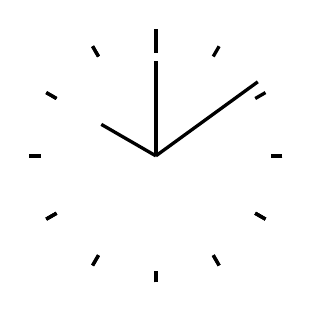
\begin{tikzpicture}
 \node[circle,minimum width=3.2cm,name=clock] at (0,0) {};
 \node[circle,minimum width=2.9cm,name=detail] at (0,0) {};
 \foreach \deg in {60,30,...,-30} {
    \draw[very thick] (clock.\deg) -- (detail.\deg);
 }
 \foreach \deg in {330,300,...,210} {
    \draw[very thick] (clock.\deg) -- (detail.\deg);
 }
 \foreach \deg in {210,180,...,120} {
    \draw[very thick] (clock.\deg) -- (detail.\deg);
 }
 \foreach \deg in {120,150,...,360} {
    \draw[very thick] (clock.\deg) -- (detail.\deg);
 }
  \draw[very thick] (clock.90) -- ++(0,-0.3);
  \draw[very thick] (clock.center) -- (150:0.8cm); % hour
  \draw[very thick] (clock.center) -- (90:1.2cm);   % minute 
  \draw[very thick] (clock.center) -- (36:1.6cm);   % second
\end{tikzpicture}
 \caption{Clock face as it would look like on the final system.}
 \label{fig:clock_face}
\end{figure}